
\documentclass[11pt]{article}
\usepackage{graphicx}
\usepackage{listings}
\usepackage{multirow}
\usepackage{color}
\usepackage[english]{babel}
\usepackage{placeins}
 \usepackage{url}
 \usepackage{mathtools}
%\usepackage{mylingmacros}

\newcommand\add[1]{{\textcolor{blue}{ADD: #1}}}
\newcommand\modi[1]{{\textcolor{green}{MODIFIED: #1}}}
\newcommand\remove[1]{{\textcolor{red}{REMOVE: #1}}}
\newcommand\expand[1]{{\textcolor{blue}{EXPAND: #1}}}
\newcommand\rewrite[1]{{\textcolor{green}{REWRITE: #1}}}

% Titre complet


\title{Data expansion for semantic classification}

\author{Anna Liednikova, Claire Gardent}


\begin{document}

\maketitle

\tableofcontents

\clearpage

\section{Introduction}

 
This project was set within the framework of a collaboration with the
ALIAE startup where the aim is to develop a chatbot to collect
information from clinical patients. The main idea is to replace
strictly defined surveys by a more natural conversation in order to
let users express themselves freely so that more information could be
collected.

The chatbot consists of three main modules: 
\begin{itemize}
\item NLU (Natura Language Understanding): interpreting the user input
\item Dialog Managment: deciding on how to respond to the user input
\item NLG: generating the system response
\end{itemize}

In this project, we focus on the NLU step which consists in
analysing the user utterance (does the user speaks about pain,
physical activity etc. ) and detecting at least one most probable
intent of user message so that later the chatbot can choose the right
strategy for fulfilling information.

\add{ADD an example showing a user input and the expected representation ie intent + entity}

A small manually annotated dataset (roughly 100 sentences for each category) was available. But that's not enough for learning a good NLU model and meet the variety of users possible inputs. Annotating sentence takes plenty of time, so some automated or semi-automated way should be chosen. So this project focuses on exploring automatic ways of extending the training data and learning NLU models from these extended data.

First, we do the literature review of approaches applied to similar problems. Later in the methodology part, we will cover four parts: building sentence representation model, evaluate it by clusterisation, train a classifier for labelling the data and application semi-supervised learning for extending the dataset. Next two our datasets and preprocessing routine will be described. Experiment part contains a quantitative and qualitative description of the models and final results. In the end, we will sum up the work have been done and give some assumption for future improvements.

\section{Literature review}

\cite{N18-2058} \modi{present an approach for automatically generating additional training data for event extraction systems}. First, they trained a baseline classifier on available data. Then, they cluster external data to obtain cluster of paraphrases using the NewsSpike method introduced by \cite{zhang2015}. They then label the clusters using the baseline model trained on the initial dataset of labelled data. Combining the new labelled data and the original one, they then retrained the event extractor.

\section{Methodology}

We follow \cite{N18-2058} methodology. Instead of using \cite{zhang2015}'s methods for identifying clusters of related sentences however, we explore different ways of representing sentences using deep learning approaches. We then apply clustering to the resulting sentence representations. Finally, we investigate the impact of the extended labeled data on classification. 

%% irst
%% group together paraphrases of event mentions.

%% then use the simple examples in each cluster to as-
%% sign a label to the entire cluster

%% com-
%% bine the new examples with the original training
%% set and retrain


\subsection{Building Sentence Representations}

We create sentence representations in two steps using machine and deep learning techniques. First, we map words to continuous representations. Second, we combine these word representations into sentence representations. 

\subsubsection{Word Representations}

We explore two ways of building word representations: Word2vec and LDA.


\paragraph{LDA.} One of the most common methods for constructing thematic models is the Latent Dirichlet Allocation (LDA) $\cite{lda_def}$. This algorithm is based on the Dirichlet prior distribution and uses in its work the bag-of-words model - a model for analyzing texts that takes into account only the frequency of words, but not their order. This model is well suited for thematic modeling, since it allows you to detect implicit relationships between words based on polysemy. The LDA method performs soft clustering and assumes that each word in the document is generated by some latent topic, which is determined by a probability distribution on the set of all words of the text.

LDA assumes the following generative process for each document \textbf{w} in a corpus \textbf{D}\cite{lda_def}:
\begin{itemize}

\item 1.Choose N $\sim$ Poisson($\xi$).
\item 2.  Choose $\theta \sim$ Dir($\alpha$).
\item 3.  For each of the N words $w_{n}$ :
\item (a)  Choose a topic $z_{n}$ $\sim$ Multinomial($\theta$).
\item (b)  Choose a word $w_{n}$ from $p(w_{n} | z_{n}, \beta)$, a multinomial probability conditioned on the topic $z_{n}$.
\end{itemize}


So finally each document with distribution vector over the topics while each topic is characterized by a distribution over words. For example,

([(0.13819554, 'sleep'),
  (0.10817484, 'morning'),
  (0.10187448, 'sometimes'),
  (0.09861754, 'help'),
  (0.060275868, 'able'),
  (0.060111083, 'nap'),
  (0.044312898, 'every'),
  (0.044219665, 'day'),
  (0.041991115, 'catch'),
  (0.04174149, 'different'),
  (0.041275226, 'many'),
  (0.041261088, 'kind'),
  (0.029845418, 'fruit'),
  (0.024193266, 'little'),
  (0.024049524, 'large'),
  (0.015836818, 'would'),
  (0.0121815335, 'bowl'),
  (0.0121815335, 'fill'),
  (0.012178916, 'salad'),
  (0.0061811106, 'hour')],
 -13.670438745757512)



\paragraph{Word2Vec.} This technology works in the following manner: word2vec takes a large text corpus as input and matches each vector with a word, producing the coordinates of the output words. First, he creates a dictionary, “learning” on the input text data, and then calculates a vector representation of the words. A vector representation is based on contextual intimacy: words that appear in the text next to identical words (and therefore, have a similar meaning) will have close coordinates of word vectors in a vector representation. The resulting word vectors can be used for natural language processing and machine learning.

$https://papers.nips.cc/paper/5021-distributed-representations-of-words-and-phrases-and-their-compositionality.pdf$

\add{example of w2v representation}

Preprocessed tokenized sentences were used to create dictionary and were passed to W2V model as it is and in form of Bag-Of-Word to LDA model.

For selecting the best model we changed space dimension (topics for LDA and features for W2W). Preferred number of features for W2V model is 200. It's the start point for our model.

The good point of using this models is that they can be used for both word and sentence representation since one word can be treated as a small sentence.


\subsubsection{Sentence Representations}

We construct sentence representations out of the word representations described in the previous section using two types of neural networks:  PositionwiseFeedForward \cite{vaswani2017attention} and BiLSTM \add{bibref}.

Here you need to explain the theory behind it. Explain how LSTM and the PositionwiseFeedForward  build a sentence representation out of word embeddings.

\paragraph{Bi-LSTM Representations.}


\subsection{Clustering Sentences}

Using the sentence representations described in the previous section, we apply clustering to group together sentences that are similar. We compare three clustering algorithms:

\begin{itemize}
\item K-Means (KM)
\item Agglomerative Clustering (AG)
\item Gaussian Mixture (GM)
\end{itemize}

We set the number of clusters to the number of intents (20)
which allows using not only purity and Silhouette coefficients to
evaluate the clusters but also homogeneity and completeness to get the
idea how resulting groups correlate with initial intents. Also, for
each model, we plot a confusion matrix with a background gradient
to visualize how well clusters separate different intents.


\paragraph{K-Means.} The basic idea is to define K centroides one for each cluster. It is best to place them as far apart as possible. The next step will be to accept each point belonging to this data set and associate it with the precision of the centroid. If no point is under consideration, the first stage is completed. At the moment, we need to re-calculate K's new centroids, as the cluster barytsentera that stems from the previous step. After these new centroids appear on us, a new binding must be made between the same points of the data set and the nearest new center of gravity. A loop is created. As a result of this cycle, we can see that k centroids change their location step by step until any changes are made. In other words, centroids are no longer moving.

The algorithm is aimed at minimizing the target function, in this case, the quadratic error function. Target function:
\begin{equation}
J = \sum_{j=1}^{k} \sum_{i=1}^{n} (\Vert x_{i}^{(j)} - c_{j} \Vert)^{2}
\end{equation}

where $(\Vert x_{i}^{(j)} - c_{j} \Vert)^{2}$ is the chosen distance between the data point $x_{i}^{(j)}$ and center $c_{j}$, it is an indicator of the distance n of the data points from their respective cluster centers.

Centroid is defined as follows:

\begin{equation}
c_{j} = \dfrac{1}{N} \sum_{i=1}^{N} x_{i}^{(j)}
\end{equation}

where $x_{i}^{(j)}$ is the point belonging to the cluster $J$, $N$ - total number of points in the cluster.

\paragraph{Agglomerative Clustering.} is a kind of hierarchical clustering with 'bottom-up' approach when new clusters are created by combining smaller clusters and, thus, a tree is created from leaves to trunk. The main feature of the agglomerative hierarchical clustering method is that if we want to get a different number of clusters, we will not need to restart the algorithm, because the whole tree is calculated, and then we say that we want to cut it in some place.


Different linkage criterions can be used to calculate distance between sets of observation. Ward’s method minimizes the variance of the clusters being merged. This method is used for tasks with closely spaced clusters. The euclidian distance between clusters is taken as the increment of the sum of squares of the distances of objects to the center of the cluster, obtained as a result of their combination: 

\begin{equation}
\Delta = \sum_{i} {(x_{i} - {\bar {x}})^{2}} - \sum_{x_{i} \in A} (x_{i} - {\bar {a}})^{2} - \sum_{x_{i} \in B} (x_{i} - {\bar {b}})^{2}
\end{equation}

At each step of the algorithm, these two clusters are combined, which lead to a minimal increase in variance.

 $Ward, Joe H. (1963). "Hierarchical Grouping to Optimize an Objective Function". Journal of the American Statistical Association. 58 (301): 236–244. doi:10.2307/2282967. JSTOR 2282967. MR 0148188.$

\paragraph{Gaussian Mixture.}

\rewrite{In statistics, a mixture model is a probabilistic model for representing the presence of subpopulations within an overall population, without requiring that an observed data set should identify the sub-population to which an individual observation belongs. Formally a mixture model corresponds to the mixture distribution that represents the probability distribution of observations in the overall population without sub-population identity information.}

A Gaussian mixture model represents a weighted sum of M Gaussian densities elements for D-dimensional continuous-valued data vectors:

\begin{equation}
p(x|\lambda) = \sum_{i=1}^{M} w_{i} g(x|\mu_{i}, \sum_{i})
\end{equation}

where each Gaussian densities element defined as 

\begin{equation}
g(x|\mu_{i}, \sum_{i})=\frac{1}{(2\pi)^{\frac{D}{2}}|\sum_{i}|^{\frac{1}{2}}} e^{-\frac{1}{2}(x-\mu_{i})'\sum_{i}(x-\mu_{i})} 
\end{equation}

with mean vector $\mu_{i}$ and covariance matrix $\sum_{i}$. The mixture weights satisfy the constraint that $\sum_{i=1}^{M} w_{i} = 1$.

GMM parameters are estimated from training data using the iterative Expectation-Maximization (EM) algorithm or Maximum A Posteriori (MAP) estimation from a well-trained prior model.

$https://pdfs.semanticscholar.org/734b/07b53c23f74a3b004d7fe341ae4fce462fc6.pdf$

\subsection{Classifying Sentences}

After choosing the best model for word embedding we train classifier to 
label data with intents. The most common approach in similar task is to use
SVC. So, we create balanced train and test dataset and validate model by 
cross validation score.

Another classical approach for classification is Random Forest Classifier.


\subsection{Semi-supervised approach}

First, we find the best clusterization for the forum data, later we classify each item and omit ones with low probability of elements at threshold Theta. In result some clusters will be empty from the beginning and some of them will be ommited due to small population.

Elements of clusters that are left will be labelled by the majority. Usually, they are pure. Later we select N labelled items for each category and extend train data with them to retrain word embedding and classificatin models.

We repeat this cycle until we won't be able to extend train dataset by additional samples or classifier score will stop to grow.

\section{Datasets}



\subsection{Labelled Data}

The initial dataset is created manually covering 20 main possible users intents. Each sentence represents one intent. For, example,

%\enumsentence{
\textbf{Text:} After sleep, for 2-3 hours, I am better and then start feeling tired again\\
\textbf{Intent:} sleep
%}

The distribution of labels is shown in Figure~\ref{figure:name}. There
are in average, 3.4 words per sentence (min: 0, max: 12, std:
2.16367).  The total number of sentences is 3305 and the vocabulary
consists of 1882 content words (after removing stopwords).

 \begin{figure}[h]
 	\centering
 	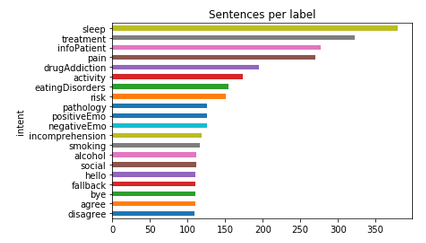
\includegraphics[scale=0.5]{report1.png}
	\caption{Label distribution in dataset}
 \label{figure:name}
 \end{figure}
\FloatBarrier



 \begin{figure}[h]
 	\centering
 	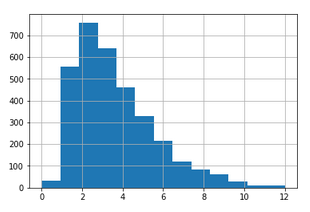
\includegraphics[scale=0.4]{report4.png}
	\caption{Sentence dist}
 \label{words_freq}
 \end{figure}
 \FloatBarrier


\subsection{Preprocessing routine}

The textual data was segmented into sentences, tokenized and lemmatized using NLP
libraries. Stop words were removed.

We compared two libraries, NLTK and SpaCy.

For example, in word tokenization they give different results that can influence not only simple statistics but meaning too. Some example of different tokenization can be seen in table \ref{token_dif}. Though concating words to ones like 'flulike' or '35mg' or 'longterm' sometimes gives more robust and concrete meaning in case of big dataset, in our case it seems better to stay with SpaCy way of tokenization in order to have smaller and more simple vocabualary.

\begin{center}
\begin{table}
\begin{tabular}{ |p{7cm}|p{7cm}| }
\hline
NLTK & SpaCy \\ \hline
['i', 'wouldnt', 'go', 'to', 'sleep', 'until', 'like', '5', '6', 'or', '8am'] & 
['i', 'would', 'nt', 'go', 'to', 'sleep', 'until', 'like', '5', '6', 'or', '8', 'am'] \\ \hline
['that', 'is', 'totally', 'wrongheaded'] & ['that', 'is', 'totally', 'wrong', 'headed'] \\ \hline
['i', 'am', 'in', 'the', 'process', 'of', 'tapering', 'from', 'suboxone', 'longterm', 'use'] & 
['i', 'am', 'in', 'the', 'process', 'of', 'tapering', 'from', 'suboxone', 'long', 'term', 'use'] \\ \hline
['i', 'had', 'an', 'onandoff', 'opiateopioid', 'habit', 'from', 'about', '2010'] & 
['i', 'had', 'an', 'on', 'and', 'off', 'opiate', 'opioid', 'habit', 'from', 'about', '2010'] \\ 
\hline
['i', 'have', 'flulike', 'pathologysymptom'] & ['i', 'have', 'flu', 'like', 'pathologysymptom'] \\ \hline
['i', 'have', 'exerciseinduced', 'insomnia'] & ['i', 'have', 'exercise', 'induced', 'insomnia'] \\ \hline
['i', 'm', 'supposed', 'to', 'take', '6', '35mg', 'tablets', 'a', 'day', 'but', 'i', 'have', 'taken', '20', 'today'] & 
['i', 'm', 'supposed', 'to', 'take', '6', '35', 'mg', 'tablets', 'a', 'day', 'but', 'i', 'have', 'taken', '20', 'today'] \\ 
\hline
\end{tabular}	
\caption{\label{token_dif}Tokenization comparison}
\end{table}
\end{center}
\FloatBarrier

For stopwords removing there were three options: nltk, spacy and the longest one. The last option was rejected due to containing words like 'want', 'stop', 'successfully' etc. that can be useful for detecting basic intents like positive or negative emotion, social. Finally nltk one was selecting because of containing shorts like 'm' from 'am', 've' from 'have'. Final dictionary contained 1882 words. Also all numbers were changed to num. Chart (\ref{words_freq}) looks fine.

 \begin{figure}[h]
 	\centering
 	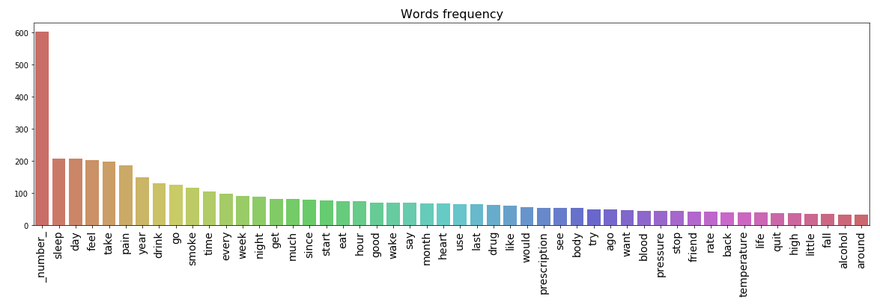
\includegraphics[scale=0.4]{report2.png}
	\caption{Words frequency}
 \label{words_freq}
 \end{figure}
\FloatBarrier

Next problem we faced is empty sentences. But there is not a lot of occurances, so their dropping don't change the dataset much.

\begin{tabular}{ |r|l| }
\hline
intent & items \\ \hline
fallback          & 12 \\ \hline
disagree          & 11 \\ \hline
hello             &  4 \\ \hline
agree             &  3 \\ \hline
incomprehension   &  2 \\ \hline
positiveEmo       &  1 \\ \hline
\end{tabular}

These sentences are: 'what?', 'same that again', 'I am up', 'same', 'can you',
       'do that', 'do this', 'Will do', 'no', 'no i will not',
       "No i don't", 'no', 'no i will not', "No i don't", "What's up?",
       "What's up?", 'he', 'a', 'd', 'i', 'm', 'o', 's', 't', 'y',
       'I will', 'Will do', 'No', 'no', 'No it is not', "No I don't",
       'No', "I'm here"


\subsection{Forum data}

We scraped 272,553 unique posts contained in each category. 

To improve initial classifier we needed to extend dataset by much more data and more naturally constracted one. No  test  set was available at the beginning of the project. To solve this  problem,  we  opted  to  created  our  own  test set following Zhang et al (2015) and Sondhi et al (2010) example.  

HealthBoards \ref{healthboards.com} is a medical forum web portal that allows patients to discuss their ailments. We scraped 272553 unique posts contained in each of 238 categories. Figure~\ref{forum_data_stat} show the dataset statistics. In average sentence contains 11+-7 words.


 \begin{figure}[h]
 	\centering
 	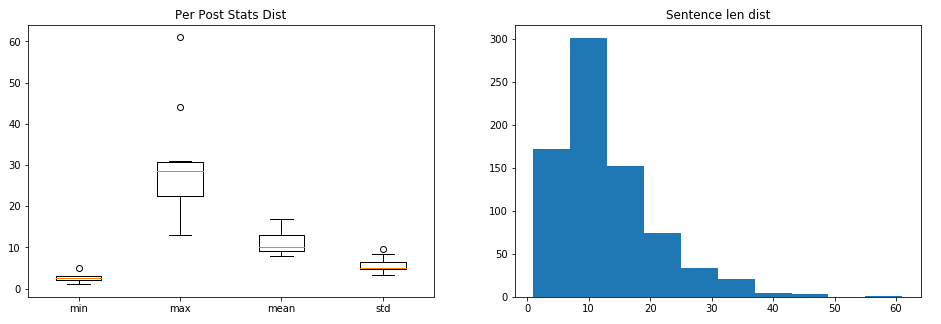
\includegraphics[scale=0.5]{report3.png}
	\caption{Text stat}\label{forum_data_stat}
 \end{figure}
\FloatBarrier


Because our intents are not that precise as forum ones we should select particular boards with relevant information to be able gradually expand their context. Result is in table \ref{cat_freq} 
We should start with the data that is most similar to the initial one, so we choose categories of boards that are similar to our intents. 

\begin{table}[htb]
\centering
\begin{tabular}{ |r|c| }
\hline
Category of board &  \# of posts \\ \hline
digestive-disorders & 5064 \\ \hline
addiction-recovery & 3644 \\ \hline
sleep-disorders & 1748 \\ \hline
smoking-cessation & 937 \\ \hline
eating-disorder-recovery & 762 \\ \hline
chronic-pain & 735 \\ \hline
chronic-fatigue & 662 \\ \hline
stress & 415 \\ \hline
family-friends-addicts-alcoholics & 312 \\ \hline
pain-management & 25 \\ \hline
\end{tabular}
\caption{\label{cat_freq}Selected categories}
\end{table}
\FloatBarrier

Finally, the corpus consists of N  sentences. 

Also, data should be divided in subsets by increasing sentence length because of the difference in mean values for both datasets. So after tokenizing posts into sentences we calculate it's length. For the each iteration we should leave sentences with mean+std words in cleaned text.


\section{Experiment}

\subsection{Clustering}

\subsubsection{Evoluation metrics}

For every model following metrics and their average were calculated: purity score, Silhouette Coefficient, homogeneity and completeness scores. Later for each parameter average among clustering models calculated for each score in order to get both table and plot.

Also for each model confusion matrix created between cluster labels and initial intents.


\subsubsection{W2V model}

Comparison table

\begin{center}
\begin{tabular}{ |c|c|c|c|c|c| }
\hline
features num & purity  & silhouette  & homogeneity  & completeness\\ \hline 
10  & 0.183157  & 0.0680834  & 0.108901  & 0.12661\\ \hline 
20  & 0.182854  & 0.0506986  & 0.111099  & 0.124805\\ \hline 
30  & \textbf{0.185477}  & 0.0683824  & 0.110799  & 0.132563\\ \hline 
50  & 0.184569  & 0.0647393  & \textbf{0.111876}  & 0.131964\\ \hline 
100  & 0.182148  & \textbf{0.0813837}  & 0.108022  & 0.138329\\ \hline 
150  & 0.183661  & 0.0298524  & 0.106401  & 0.141179\\ \hline 
200  & 0.176803  & 0.0581627  & 0.103708  & 0.141973\\ \hline 
300  & 0.176097  & 0.0432732  & 0.106379  & 0.151118\\ \hline 
400  & 0.169642  & 0.0626822  & 0.100455  & 0.148768\\ \hline 
500  & 0.168533  & 0.0653733  & 0.0976706  & 0.146799\\ \hline 
550  & 0.17176  & 0.0584935  & 0.0994422  & \textbf{0.151185}\\ \hline 
600  & 0.169138  & 0.0574187  & 0.0980455  & 0.150695\\ \hline \end{tabular}
\end{center}
\FloatBarrier

\begin{figure}[h]
\centering
 	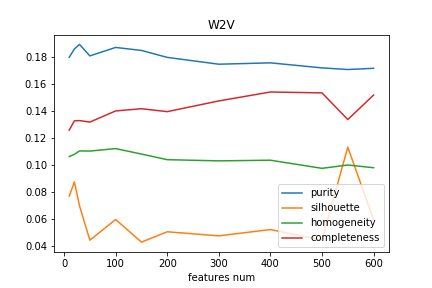
\includegraphics[scale=0.7]{w2v_scores.png}
	\caption{LDA scores}
\label{w2v_scores}
\end{figure}
\FloatBarrier

Later we will try both 10 and 100 features.

\begin{figure}[h]
	\centering
 	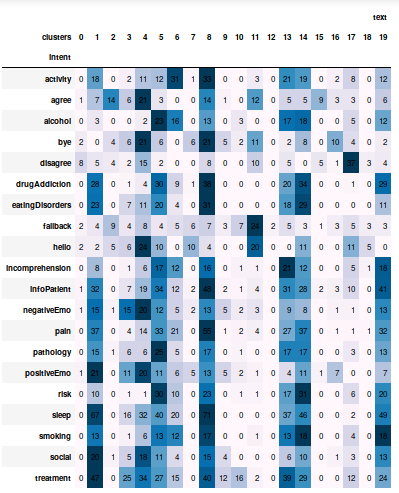
\includegraphics[scale=0.7]{best_w2v_cm.png}
	\caption{W2V confusion matrix}
 \label{w2v_cm_mat}
 \end{figure}
\FloatBarrier

\subsubsection{LDA model}

\begin{center}
\begin{tabular}{ |c|c|c|c|c| }
\hline
num & purity  & silhouette  & homogeneity  & completeness \\ \hline 
10  & 0.253656  & 0.461589  & 0.157498  & 0.178928  \\ \hline 
20  & 0.259203  & 0.378276  & 0.168191  & 0.182203  \\ \hline 
30  & 0.251538  & 0.331069  & 0.157755  & 0.168448  \\ \hline 
50  & 0.240545  & 0.287032  & 0.147430  & 0.166824  \\ \hline 
100  & 0.266465  & 0.187596  & 0.168647  & 0.189221 \\ \hline 
150  & 0.256077  & 0.167888  & 0.161589  & 0.185054 \\ \hline 
200  & 0.263843  & 0.149212  & 0.175117  & \textbf{0.194913} \\ \hline 
300  & 0.250025  & 0.151526  & 0.165607  & 0.184314 \\ \hline 
400  & \textbf{0.272718}  & 0.192777  & \textbf{0.177547}  & 0.192270 \\ \hline 
500  & 0.259506  & \textbf{0.203725}  & 0.174925  & 0.192831 \\ \hline 
550  & 0.229450  & 0.166200  & 0.149270  & 0.158548 \\ \hline 
600  & 0.254261  & 0.191729  & 0.171744  & 0.186001 \\
\hline 
\end{tabular}
\end{center}
\FloatBarrier

\begin{figure}[h]
 	\centering
 	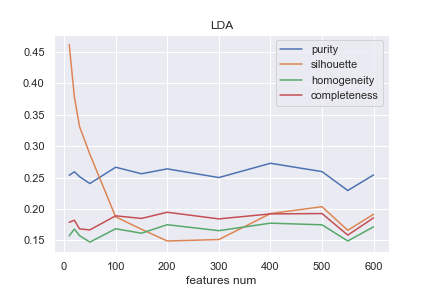
\includegraphics[scale=0.7]{lda_scores.png}
	\caption{LDA scores}
\label{lda_scores}
\end{figure}
\FloatBarrier

The best model - is LDA with 400 topics according to scores and with priority to purity and homogeneity ones.

Thanks to confusion matrix that is constructed based on cluster and intent labels we can make assumpsions about possible errors and difficulties and figure out what connections our model distinguish well. Though different clustering algorithms still captures different connection between intents, there are some common groups for all of them: fallback and hello; alcohol, drugAddiction and risk; social and emotions.


\begin{figure}[h]
	\centering
	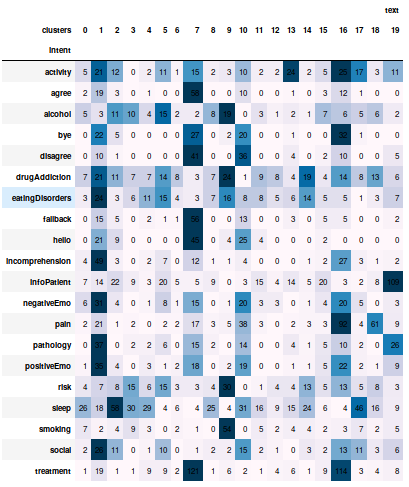
\includegraphics[scale=0.7]{lda_gm_cm.png}
	\caption{LDA confusion matrix for gaussian mixture}
\label{lda_gm_cm}
\end{figure}
\FloatBarrier


\subsubsection{GloVe pretrained}

\subsubsection{Google News W2V pretrained}

We used word2vec google-news model with 300 dimensional feature space.


CV 0.418 + 0.057%

\subsubsection{CNN by word}

From simple encoder, w2v, lda, w2v + lda

\subsubsection{BiLSTM by word}

From simple encoder, w2v, lda, w2v + lda

\centering
\begin{tabular}{ |r|c|c|c|c|c| }
\hline
layers & purity  & silhouette  & homogeneity  & completeness \\ \hline 
1  & \textbf{0.286369}  & 0.239979  & \textbf{0.227069}  & \textbf{0.232338}\\ \hline 
2  & 0.262836  & 0.181804  & 0.211068  & 0.219279\\ \hline 
3  & 0.238284  & 0.266460  & 0.195002  & 0.206703\\ \hline 
4  & 0.218623  & \textbf{0.439161}  & 0.164478  & 0.192599
\end{tabular}
\FloatBarrier

So it's better to stay with one layer.

\centering
\begin{tabular}{ |r|c|c|c|c|c| }
\hline
layers & purity  & silhouette  & homogeneity  & completeness \\ \hline 
32  & 0.270273  & 0.244798  & 0.214607  & 0.21474\\ \hline 
64  & \textbf{0.281683}  & 0.22728  & 0.231666  & 0.232176\\ \hline 
128  & 0.271597  & 0.263519  & \textbf{0.234111}  & \textbf{0.235486}\\ \hline 
256  & 0.270681  & 0.267634  & 0.229275  & 0.231675\\ \hline 
512  & 0.277608  & 0.264844  & 0.231268  & 0.235075\\ \hline 
1024  & 0.266707  & 0.260425  & 0.226291  & 0.229238\\ \hline 
2048  & 0.268796  & \textbf{0.278391}  & 0.228211  & 0.231041 \\ \hline
\end{tabular}
\FloatBarrier

64 output size due to bigger difference in purity score

With maxpool on hidden layer
\centering
\begin{tabular}{ |r|c|c|c|c|c| }
\hline
layers & purity  & silhouette  & homogeneity  & completeness \\ \hline 
64 &	0.272616 	& 0.177766 	& 0.218339 	& 0.219109 \\ \hline
\end{tabular}
\FloatBarrier

With maxpool on output
\centering
\begin{tabular}{ |r|c|c|c|c|c| }
\hline
layers & purity  & silhouette  & homogeneity  & completeness \\ \hline 
64 	& 0.256011 	& 0.183609 	& 0.200849 	& 0.20462 \\ \hline
\end{tabular}
\FloatBarrier

BiLSTM model with one 64-dimensional layer without pooling.

\subsubsection{Overall comparison}

\centering
\begin{tabular}{ |r|c|c|c|c|c| }
\hline
model & features & purity  & silhouette  & homogeneity  & completeness \\ \hline 
W2V 	& 10   & 0.192032  & 0.077404  & 0.108761  & 0.127672 \\ \hline 
W2V 	& 100  & 0.184266  & 0.065381  & 0.109944  & 0.144074 \\ \hline 
LDA 	& 400  & 0.272718  & 0.192777  & 0.177547  & 0.192270 \\ \hline 
BiLSTM 	& 64  & \textbf{0.281683}  & 0.22728  & 0.231666  & 0.232176\\ \hline 
\end{tabular}
\FloatBarrier



\subsection{Classifier}

\subsubsection{Evoluation metrics}



\subsubsection{Results for each model}

\subsection{Semi-supervised learning}

\section{Conclusion}


\section{References}
\bibliographystyle{alpha}
\bibliography{biblio}
$ Ward J.H. Hierarchical grouping to optimize an objective function // J. of the American Statistical Association, 1963. — 236 р. $

\end{document}
